\section{Model fits and model comparison}
\label{sec:models}

In the experiments reported above, we see strong evidence that participants are engaging in reasoning that goes beyond the simple semantic interpretation of messages. Instead, they appear to be making inferences about reference in context that have the character of pragmatic reasoning---considering inferential alternatives that a speaker could have said. In this section, we test the ability of the RSA model to describe human behavior in these experiments. 

We are well aware of the difficulties surrounding reasoning from a good fit alone \cite{roberts2000}. In a nutshell, any model must both show that it \emph{can} predict the data that actually occurred and \emph{cannot} predict the data that did not occur. The flexibility of the theory is thus of critical importance in understanding its performance. The RSA model as stated here and earlier contains a relatively small number of parameters, however: primarily $n$ (the depth of recursion) and $\alpha$, the greed parameter in the choice rule. 

 \begin{figure}[t]
  \centering
  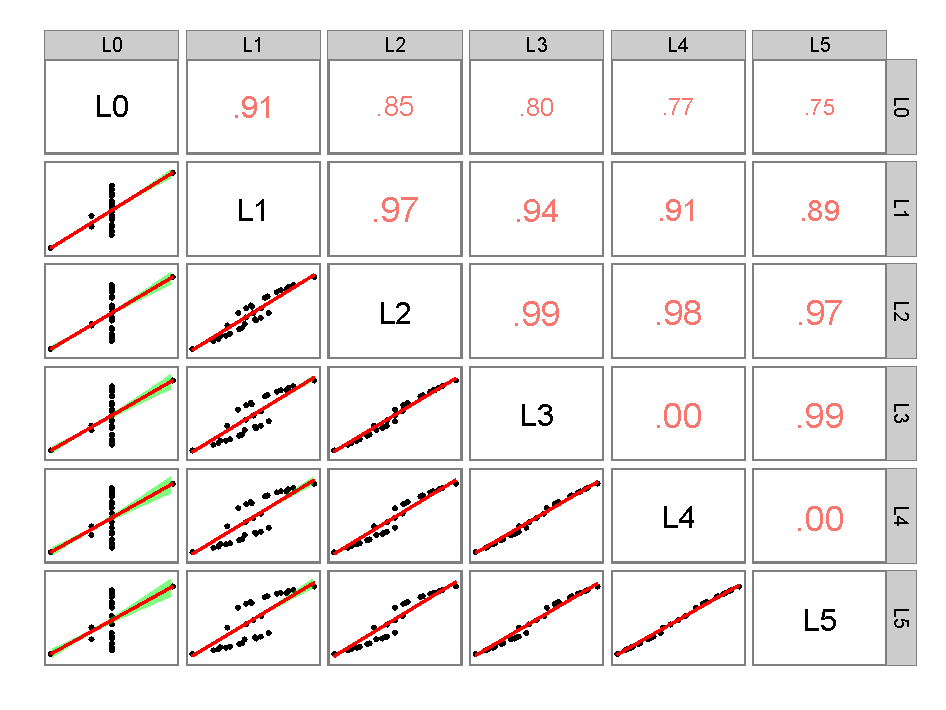
\includegraphics[width=6in]{../plots/models-2.pdf}
  \caption{\label{fig:models-2} Model identifiability simulation results. Each plot on the lower triangle shows model predictions for one model plotted by predictions for another. Each dot is an experimental condition, with trend lines showing simple linear regression with 95\% confidence intervals. Each plot on the upper triangle shows the pearson correlation value between those two models. Models with higher levels of recursion are very difficult to distinguish from one another.}
\end{figure}


 \begin{figure}[t]
  \centering
  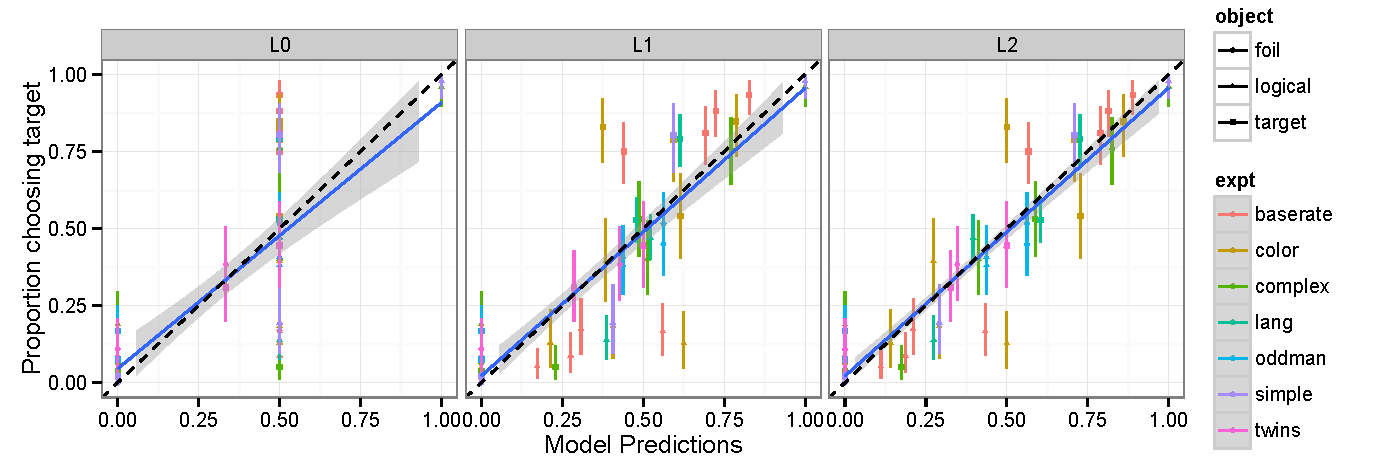
\includegraphics[width=6in]{../plots/models-1.pdf}
  \caption{\label{fig:models-2} Full model fit to data for $L_0$, $L_1$, and $L_2$. Each point represents proportions choosing a particular target object in an experimental condition. The diagonal dashed line shows perfect fit, and the blue solid line shows a line of best fit with 95\% confidence intervals.}
\end{figure}

In our first analysis, we 


\subsection{Identifiability}

%%% Local Variables: 
%%% TeX-master: "pragmods"
%%% End:
